\subsection{\href{http://www.koner.com.ar/}{Grupo Koner}}
   \hypertarget{subsec:koner}
   Para la empresa Grupo Koner se desarrolló y customizó un lector RFID para el registro y control de accesos de los conductores de las flotas de vehículos monitoreados.\\
   Por otro lado se diseño y construyó un equipo inalámbrico para la integración entre radio controles y el rastreador del vehículo permitiendo evitar el cableado de botoneras.
   \begin{figure}
      \begin{center}
         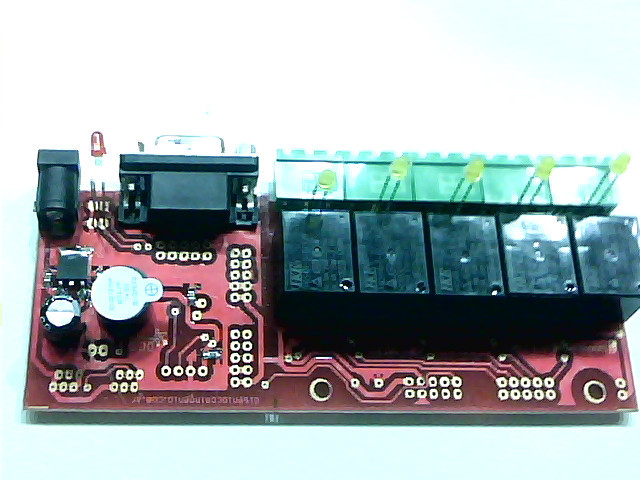
\includegraphics[width=0.24\textwidth]{portfolio/xenon4.jpg}
         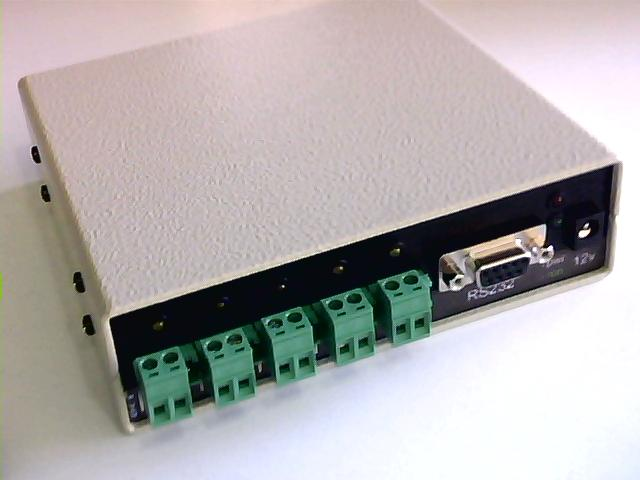
\includegraphics[width=0.24\textwidth]{portfolio/xenon1.jpg}
         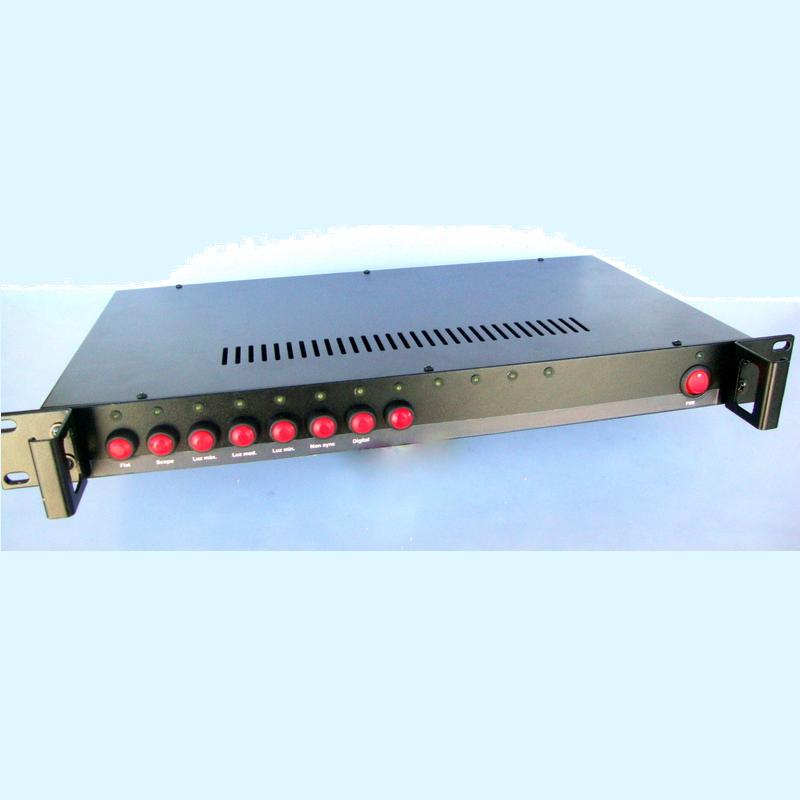
\includegraphics[width=0.24\textwidth]{portfolio/xenon2.jpg}
         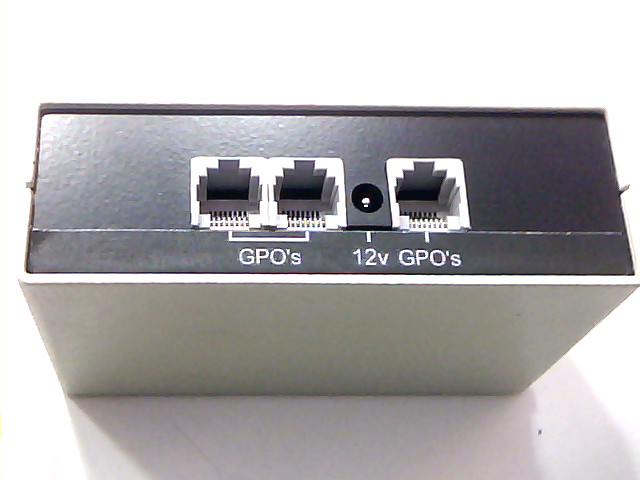
\includegraphics[width=0.24\textwidth]{portfolio/xenon3.jpg}
      \end{center}
      \caption{Equipo inalámbrico de integración entre el rastreador AVL y radio controles.}
      \label{fig:koner}
   \end{figure}
